\subsection{Temporal Accuracy Assessment}
\label{subsec:temporal_accuracy}

Temporal accuracy is assessed through a self-convergence study
in which the spatial grid and integration horizon are kept
fixed while the pseudo-time step is successively reduced.
For each time step, the solver advances the initial temperature
field over the same total pseudo-time interval. This allows
the differences between the resulting temperature fields to
be attributed primarily to temporal discretization.

The computational domain is discretized using a fixed grid
of $25\times10$ cells. The initial time step is
$\Delta t_0=0.05$, and three successive halvings are applied,
giving four time-step levels:
\begin{equation}
\Delta t_\ell=\frac{\Delta t_0}{2^\ell},
\qquad \ell=0,1,2,3.
\label{eq:temporal_step_refinement}
\end{equation}

All calculations are performed over the same final pseudo-time
$\tau_f=0.5$. Consequently, the required number of iterations
for each time step is
\begin{equation}
N_\ell=\frac{\tau_f}{\Delta t_\ell},
\label{eq:temporal_iteration_count}
\end{equation}
which gives $10$, $20$, $40$, and $80$ iterations,
respectively.

To ensure that every calculation reaches the same integration
horizon, residual-based early termination is disabled by
setting the residual tolerance to zero. The maximum iteration
count is set equal to the required number of time steps, and
the actual number of iterations is checked after each run.

\subsubsection{Successive-Time-Step Differences}

Since all solutions are obtained on the same spatial grid,
their physical-cell temperature fields can be compared
directly, without spatial interpolation. Ghost cells are
excluded from the comparison.

The RMS difference between solutions obtained using two
successive time steps is defined as
\begin{equation}
D_{\ell,\ell+1}
=
\sqrt{
\frac{1}{n_xn_y}
\sum_{i=1}^{n_x}
\sum_{j=1}^{n_y}
\left(
T_{ij}^{\Delta t_\ell}
-
T_{ij}^{\Delta t_{\ell+1}}
\right)^2
},
\label{eq:temporal_difference_norm}
\end{equation}
where both solutions correspond to the same final pseudo-time
and spatial grid.

\subsubsection{Observed Temporal Convergence Order}

Assuming that the numerical solutions are in the asymptotic
temporal convergence range, the successive-time-step
differences approximately satisfy
\begin{equation}
D_{\ell,\ell+1}\propto(\Delta t_\ell)^p,
\label{eq:temporal_difference_scaling}
\end{equation}
where $p$ is the observed temporal order of convergence.

Since each time-step refinement reduces $\Delta t$ by a
factor of two, the observed order between successive
difference estimates is
\begin{equation}
\boxed{
p_{\mathrm{obs},\ell}
=
\frac{
\ln\left(D_{\ell,\ell+1}/D_{\ell+1,\ell+2}\right)
}{
\ln 2
}.
}
\label{eq:observed_temporal_order}
\end{equation}

In addition to the pairwise estimates, a fitted temporal
order is obtained through a least-squares linear fit of
$\ln D_{\ell,\ell+1}$ against $\ln\Delta t_\ell$:
\begin{equation}
\ln D_{\ell,\ell+1}
=
p_{\mathrm{fit}}\ln\Delta t_\ell+C,
\label{eq:temporal_log_fit}
\end{equation}
where $p_{\mathrm{fit}}$ is the fitted slope and $C$ is
the intercept.

\begin{algorithm}[H]
\caption{Temporal Self-Convergence Analysis}
\label{alg:temporal_self_convergence}
\begin{algorithmic}[1]
\Require Fixed mesh $M$, initial time step $\Delta t_0$,
number of time-step levels $N_{\Delta t}=4$, final
pseudo-time $\tau_f$, solver, and physical parameters
\Ensure Successive-time-step differences, observed and
fitted temporal orders, and convergence diagnostics

\State Generate the time-step sequence using
Equation~\eqref{eq:temporal_step_refinement}
\State Initialize solution and diagnostic records

\For{each time step $\Delta t_\ell$}
    \State Calculate the required iteration count
    $N_\ell$ using Equation~\eqref{eq:temporal_iteration_count}
    \State Initialize the temperature and velocity fields
    on the fixed mesh
    \State Set residual tolerance to zero and maximum
    iterations to $N_\ell$
    \State Execute the selected solver
    \State Verify that exactly $N_\ell$ iterations were performed
    \State Check that the final temperature field contains
    only finite values
    \State Store the final temperature field, residual,
    iteration count, and computation time
\EndFor

\For{each pair of successive time steps}
    \State Extract physical-cell temperatures from both solutions
    \State Calculate the RMS difference using
    Equation~\eqref{eq:temporal_difference_norm}
    \State Store the resulting difference
\EndFor

\For{each pair of successive difference estimates}
    \State Calculate the observed temporal order using
    Equation~\eqref{eq:observed_temporal_order}
\EndFor

\State Fit $\ln D_{\ell,\ell+1}$ against
$\ln\Delta t_\ell$ using least squares
\State Record the fitted slope $p_{\mathrm{fit}}$
\State Generate the log--log temporal self-convergence plot
\State Save time steps, differences, observed orders,
fitted order, residuals, iteration counts, and computation times
\State \Return temporal convergence results and diagnostics
\end{algorithmic}
\end{algorithm}

The temporal self-convergence study provides an estimate of
the time-integration accuracy without requiring an exact
transient solution. Its reliability depends on comparing
solutions at the same integration horizon, using sufficiently
fine time steps to reach the asymptotic convergence range.

\subsubsection{Temporal Accuracy Results}
\label{subsec:temporal_accuracy_results}

The temporal accuracy of the four numerical methods was
assessed on a fixed $25\times10$ spatial grid using
$\mathrm{Pe}=17.5$, $\mathrm{Br}=0.2$, and a linear inlet
temperature profile $T_{\mathrm{in}}(y)=y$. All calculations
were advanced over the same final pseudo-time $\tau_f=0.5$,
using successively halved time steps:
\begin{equation}
\Delta t=
\{0.05,\;0.025,\;0.0125,\;0.00625\}.
\end{equation}

The residual-based steady-state termination criterion was
disabled to ensure that all solutions were evaluated at the
same integration horizon. Consequently, the calculations
were performed for exactly $10$, $20$, $40$, and $80$
iterations, respectively.

The successive-time-step RMS differences and the resulting
temporal convergence orders are summarized in
Table~\ref{tab:temporal_accuracy_results}.

\begin{table}[H]
\centering
\caption{Temporal self-convergence results for the four
numerical methods.}
\label{tab:temporal_accuracy_results}
\small
\setlength{\tabcolsep}{5pt}
\renewcommand{\arraystretch}{1.3}
\resizebox{\textwidth}{!}{%
\begin{tabular}{c c c c c c c}
\hline
Method
& $D_{0,1}$
& $D_{1,2}$
& $D_{2,3}$
& $p_{\mathrm{obs},1}$
& $p_{\mathrm{obs},2}$
& $p_{\mathrm{fit}}$
\\
\hline
APF
& $4.8819\times10^{-3}$
& $2.5673\times10^{-3}$
& $1.3341\times10^{-3}$
& 0.92721
& 0.94437
& 0.93579
\\

RK2
& $9.3241\times10^{-4}$
& $2.1548\times10^{-4}$
& $5.2779\times10^{-5}$
& 2.11338
& 2.02955
& 2.07147
\\

RK4
& $2.0929\times10^{-5}$
& $1.2419\times10^{-6}$
& $7.5599\times10^{-8}$
& 4.07489
& 4.03803
& 4.05646
\\

Direct
& $4.7960\times10^{-3}$
& $2.5499\times10^{-3}$
& $1.3306\times10^{-3}$
& 0.91137
& 0.93840
& 0.92488
\\
\hline
\end{tabular}%
}
\end{table}

Here, $D_{0,1}$, $D_{1,2}$, and $D_{2,3}$ denote the
RMS differences between solutions obtained using successive
time steps. The observed orders are calculated using
Equation~\eqref{eq:observed_temporal_order}, while
$p_{\mathrm{fit}}$ represents the slope of the corresponding
log--log least-squares fit.

\begin{figure}[H]
\centering

\begin{minipage}[t]{0.48\textwidth}
    \centering
    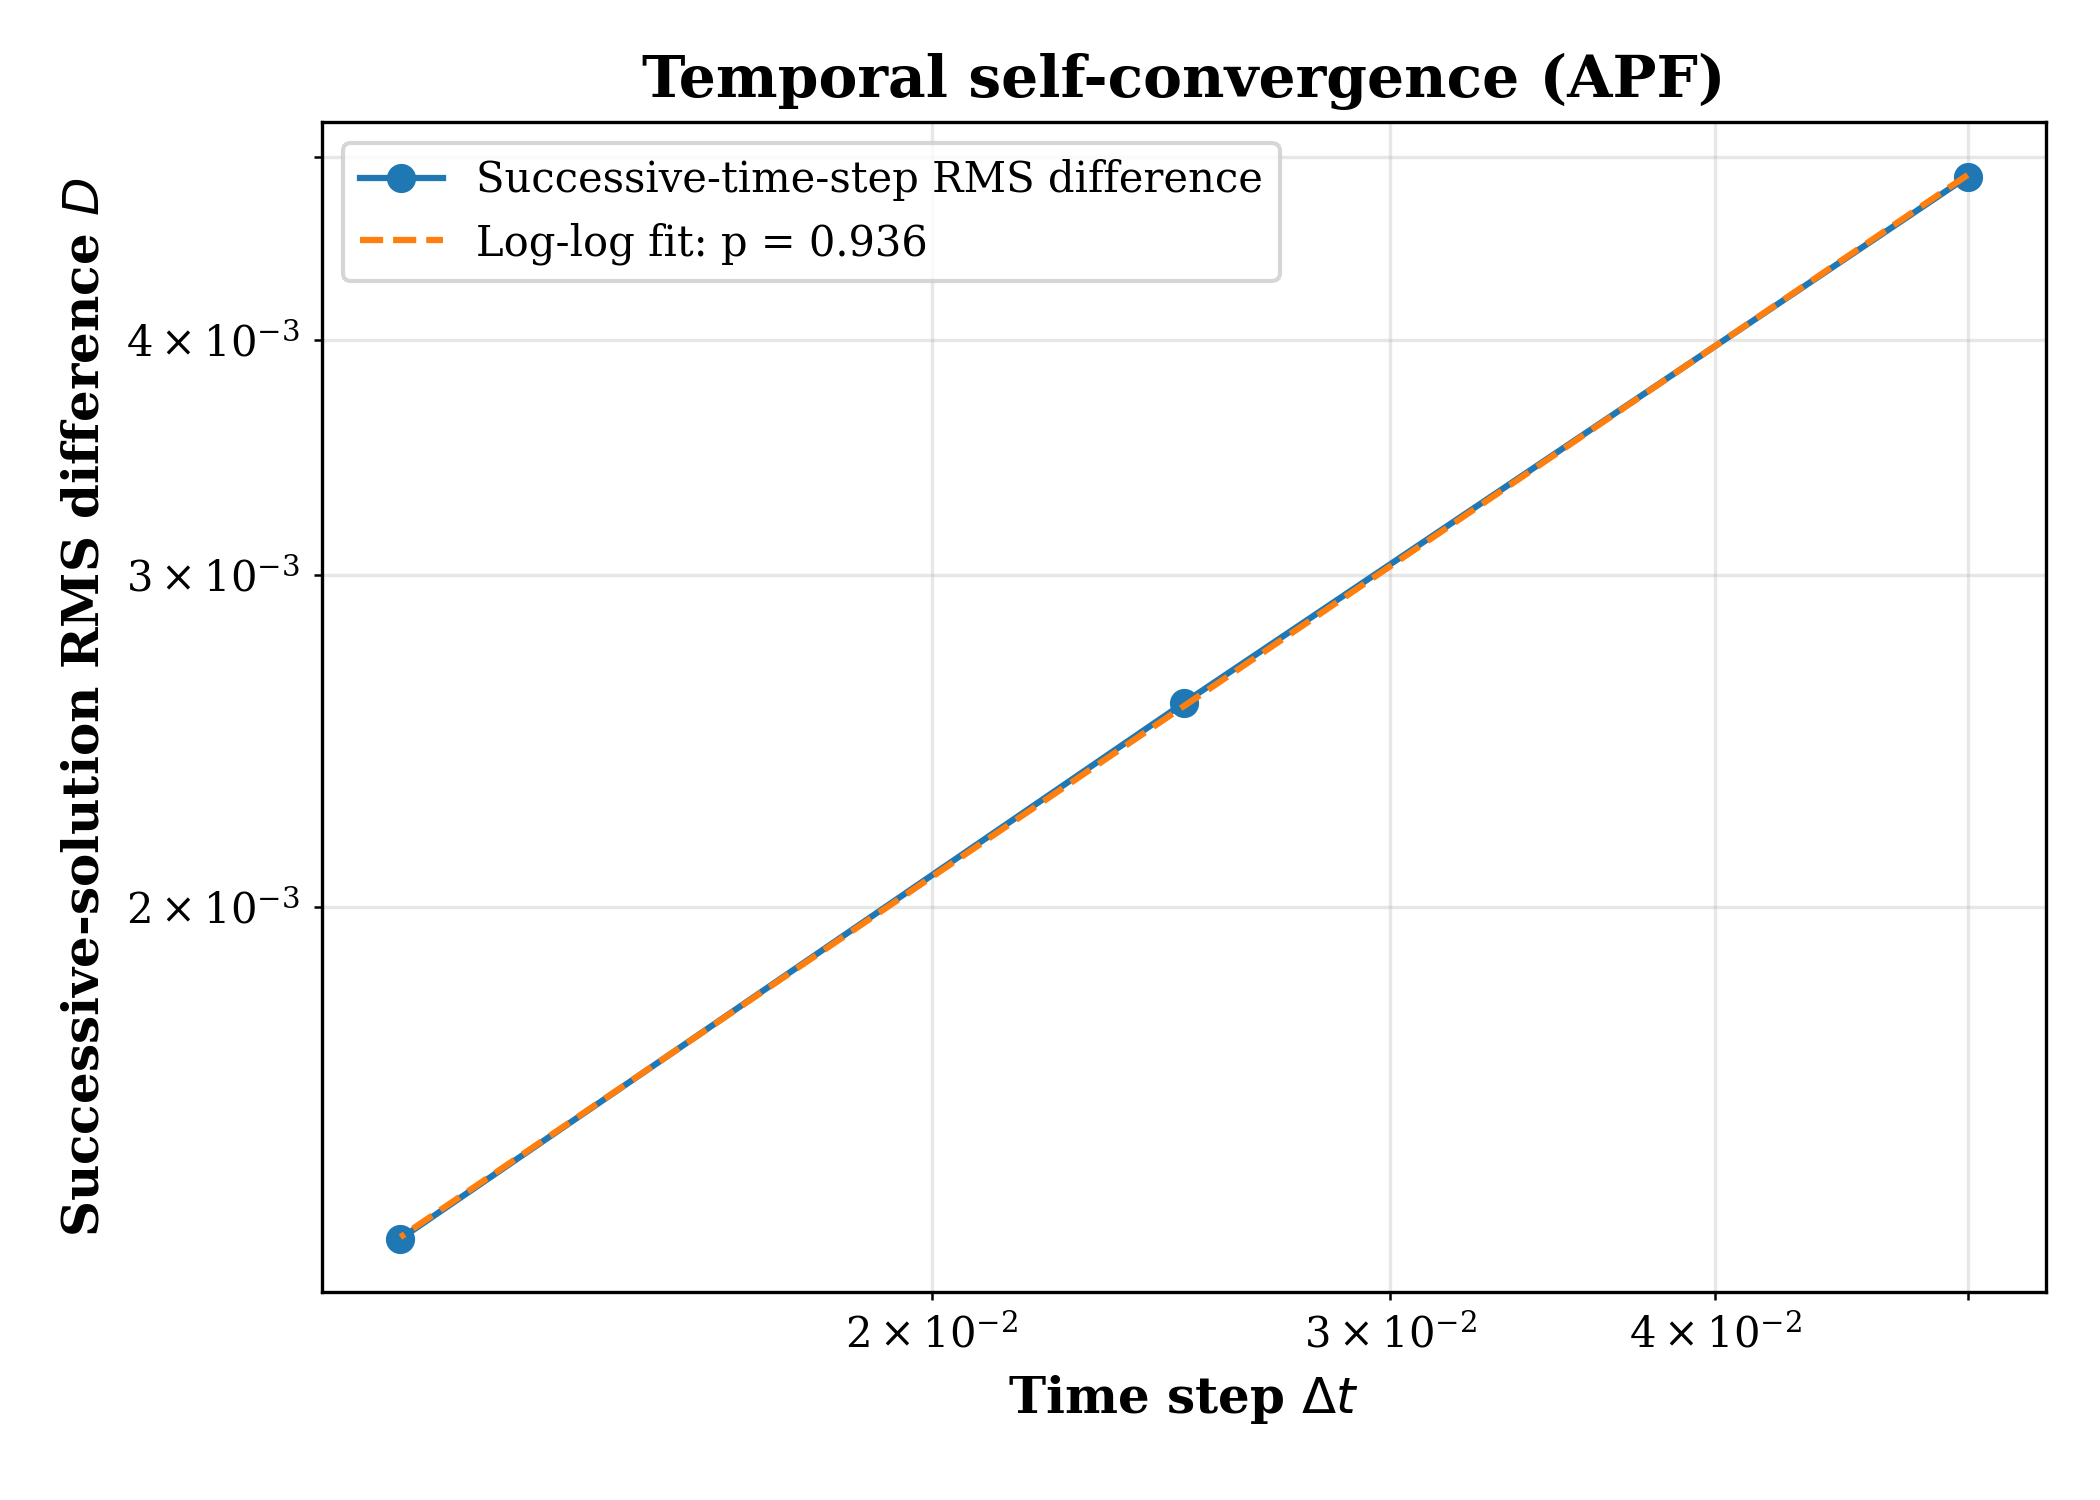
\includegraphics[width=\linewidth]
    {figures/temporal_self_convergence_APF.png}

    {\small (a) Approximate factorization (APF)}
\end{minipage}
\hfill
\begin{minipage}[t]{0.48\textwidth}
    \centering
    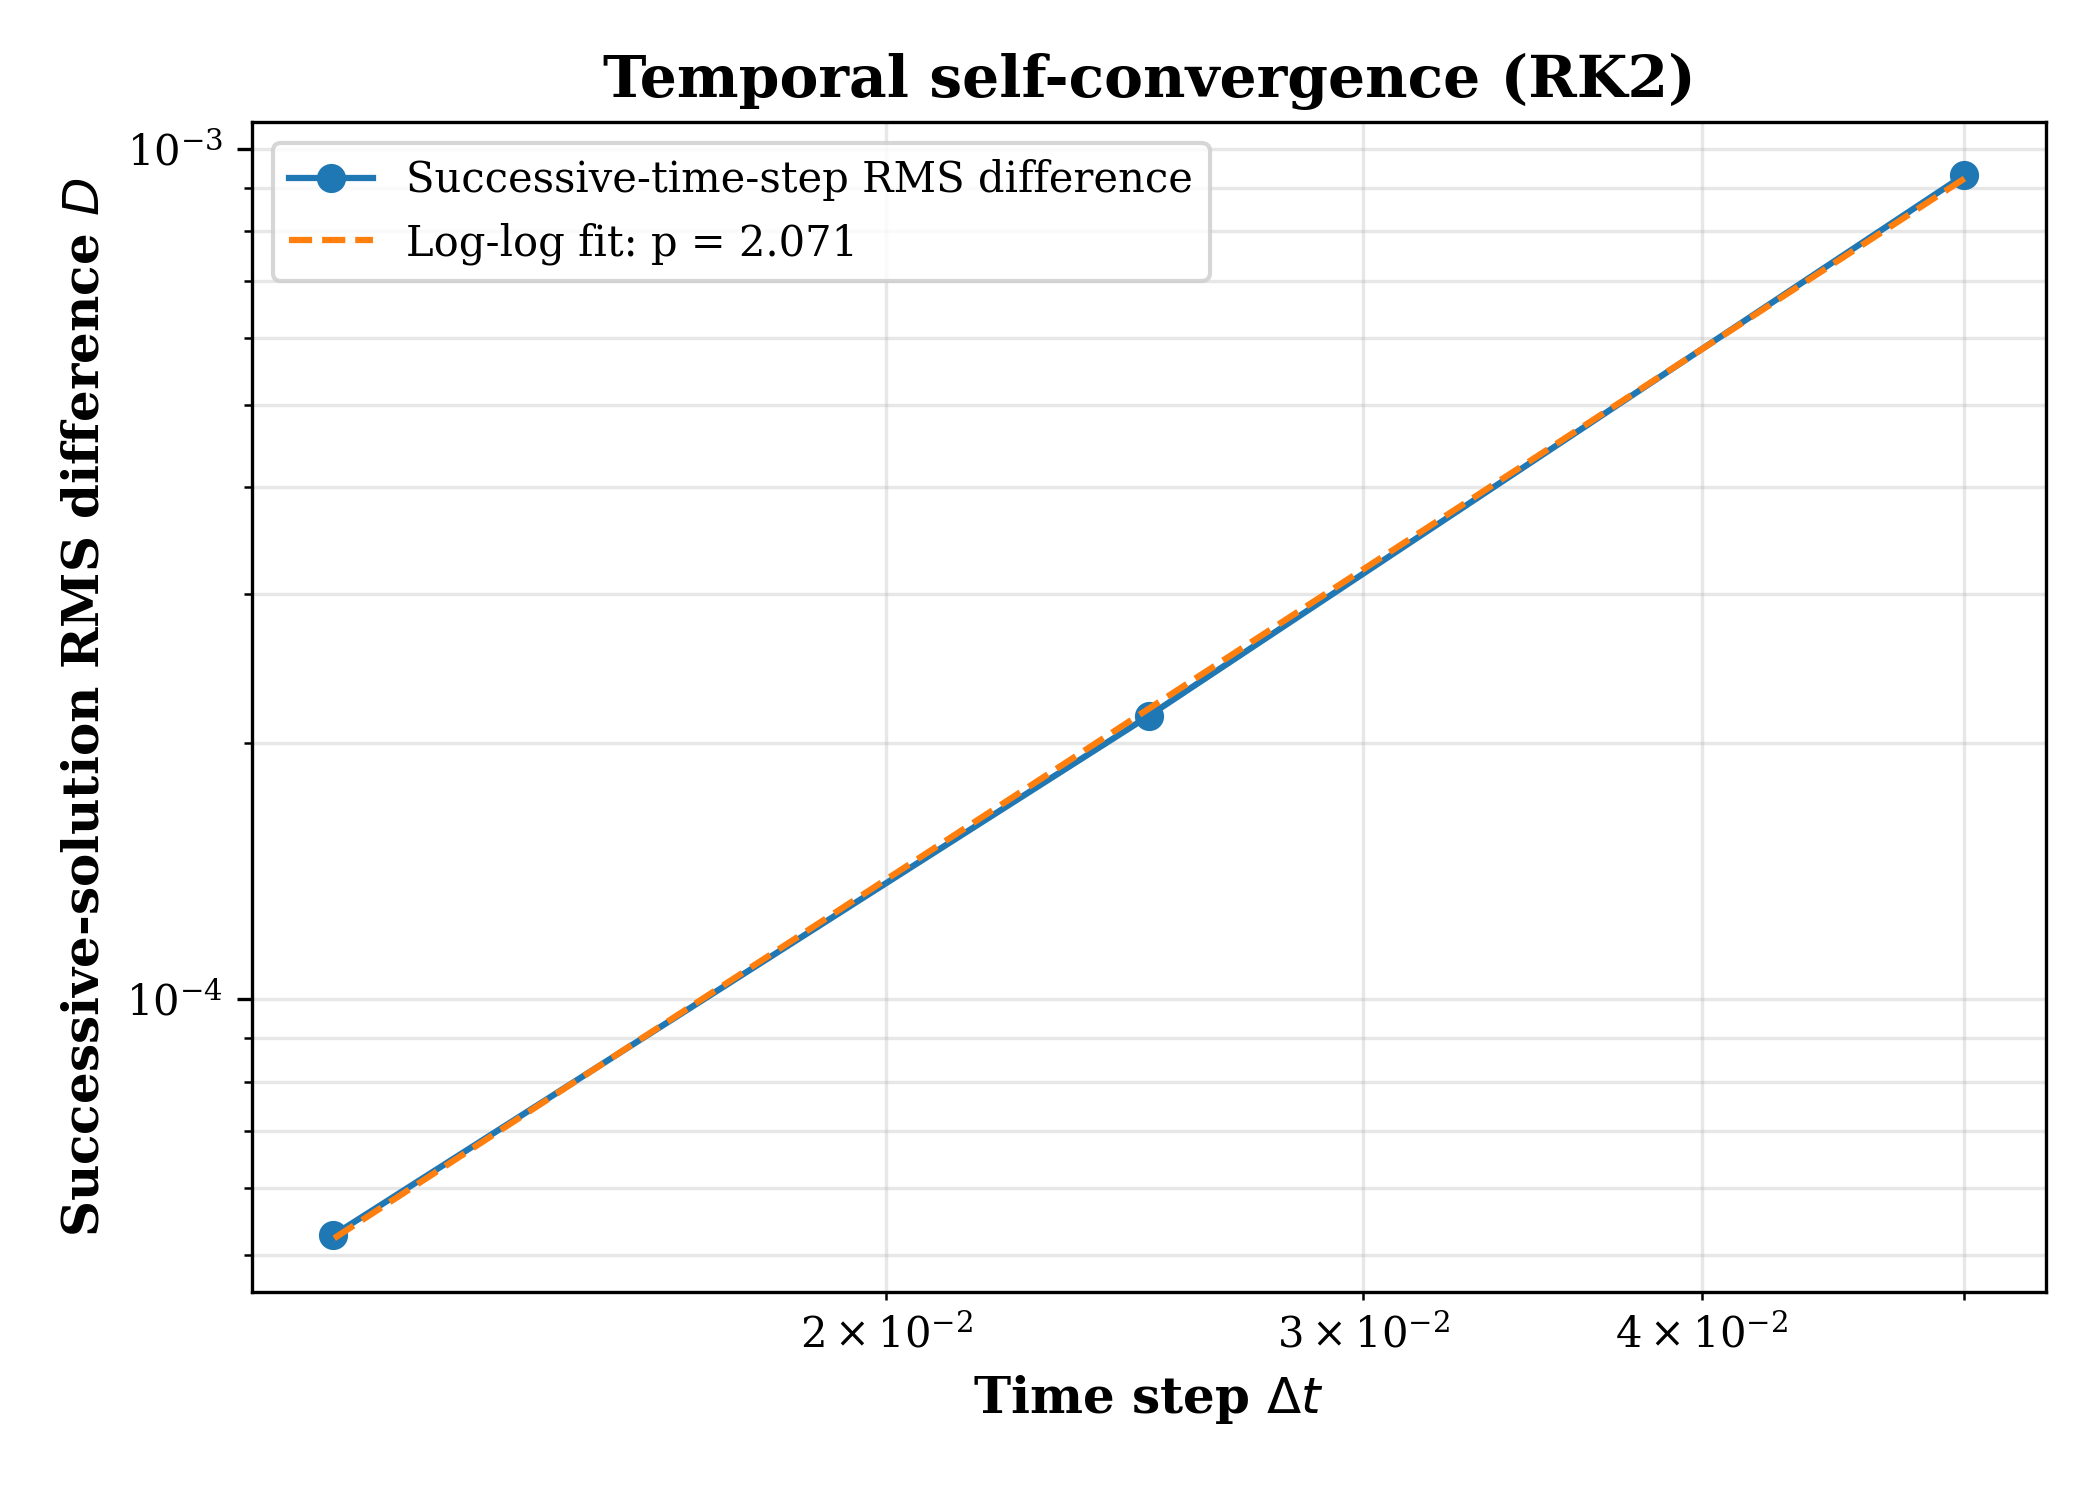
\includegraphics[width=\linewidth]
    {figures/temporal_self_convergence_RK2.png}

    {\small (b) Explicit midpoint RK2}
\end{minipage}

\vspace{0.4cm}

\begin{minipage}[t]{0.48\textwidth}
    \centering
    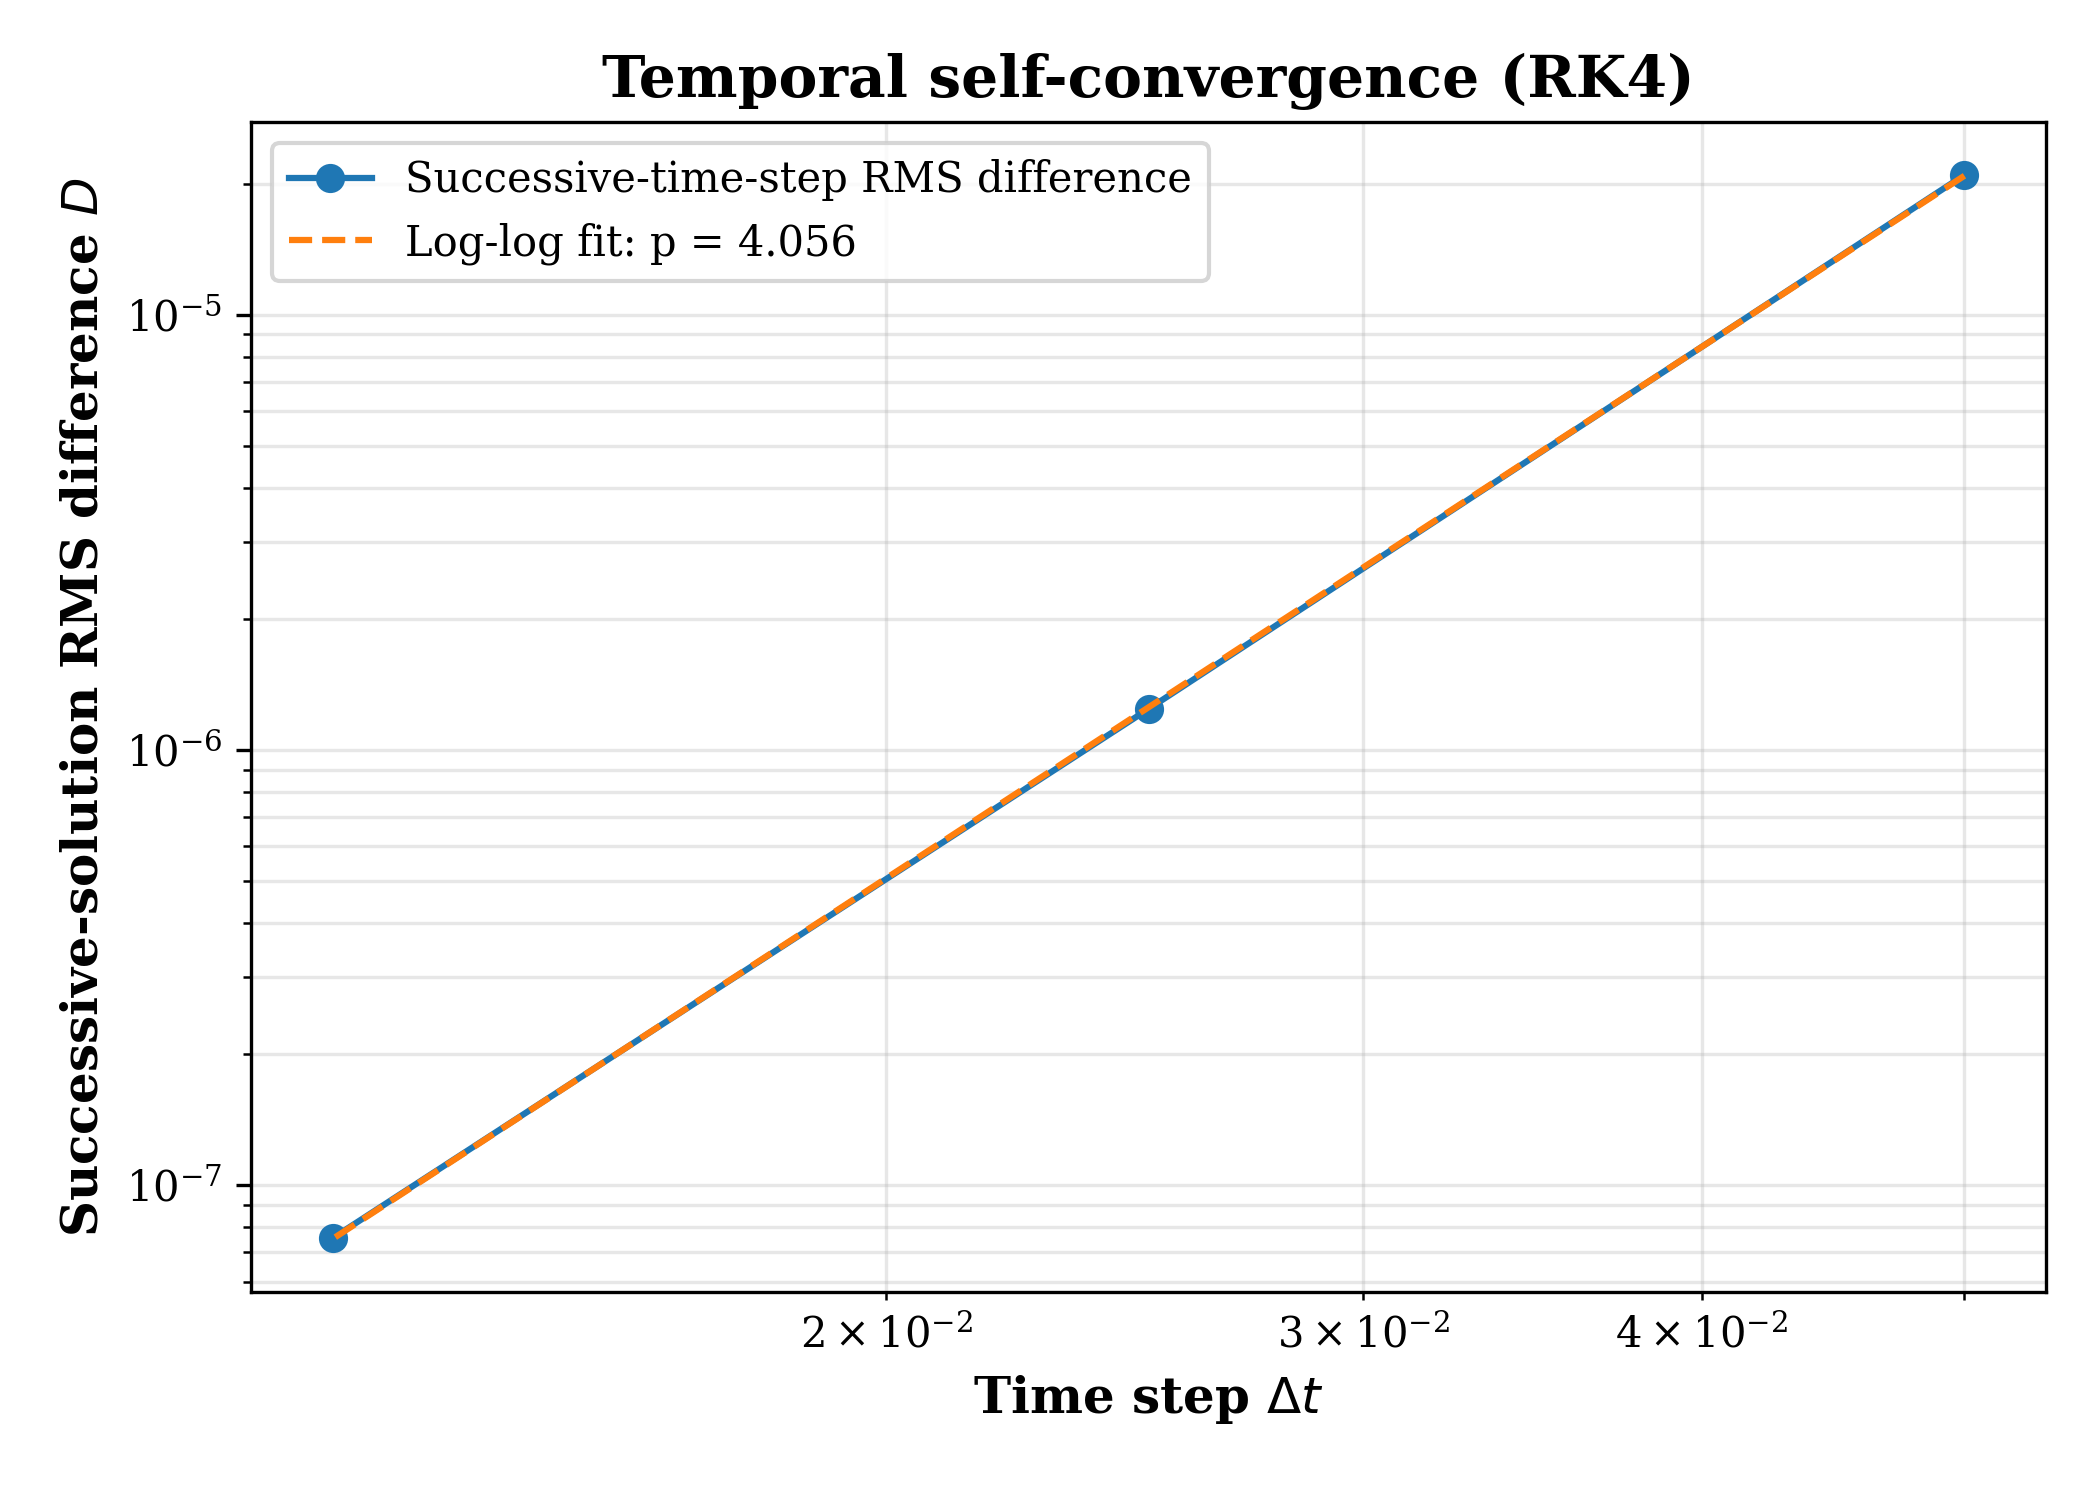
\includegraphics[width=\linewidth]
    {figures/temporal_self_convergence_RK4.png}

    {\small (c) Classical RK4}
\end{minipage}
\hfill
\begin{minipage}[t]{0.48\textwidth}
    \centering
    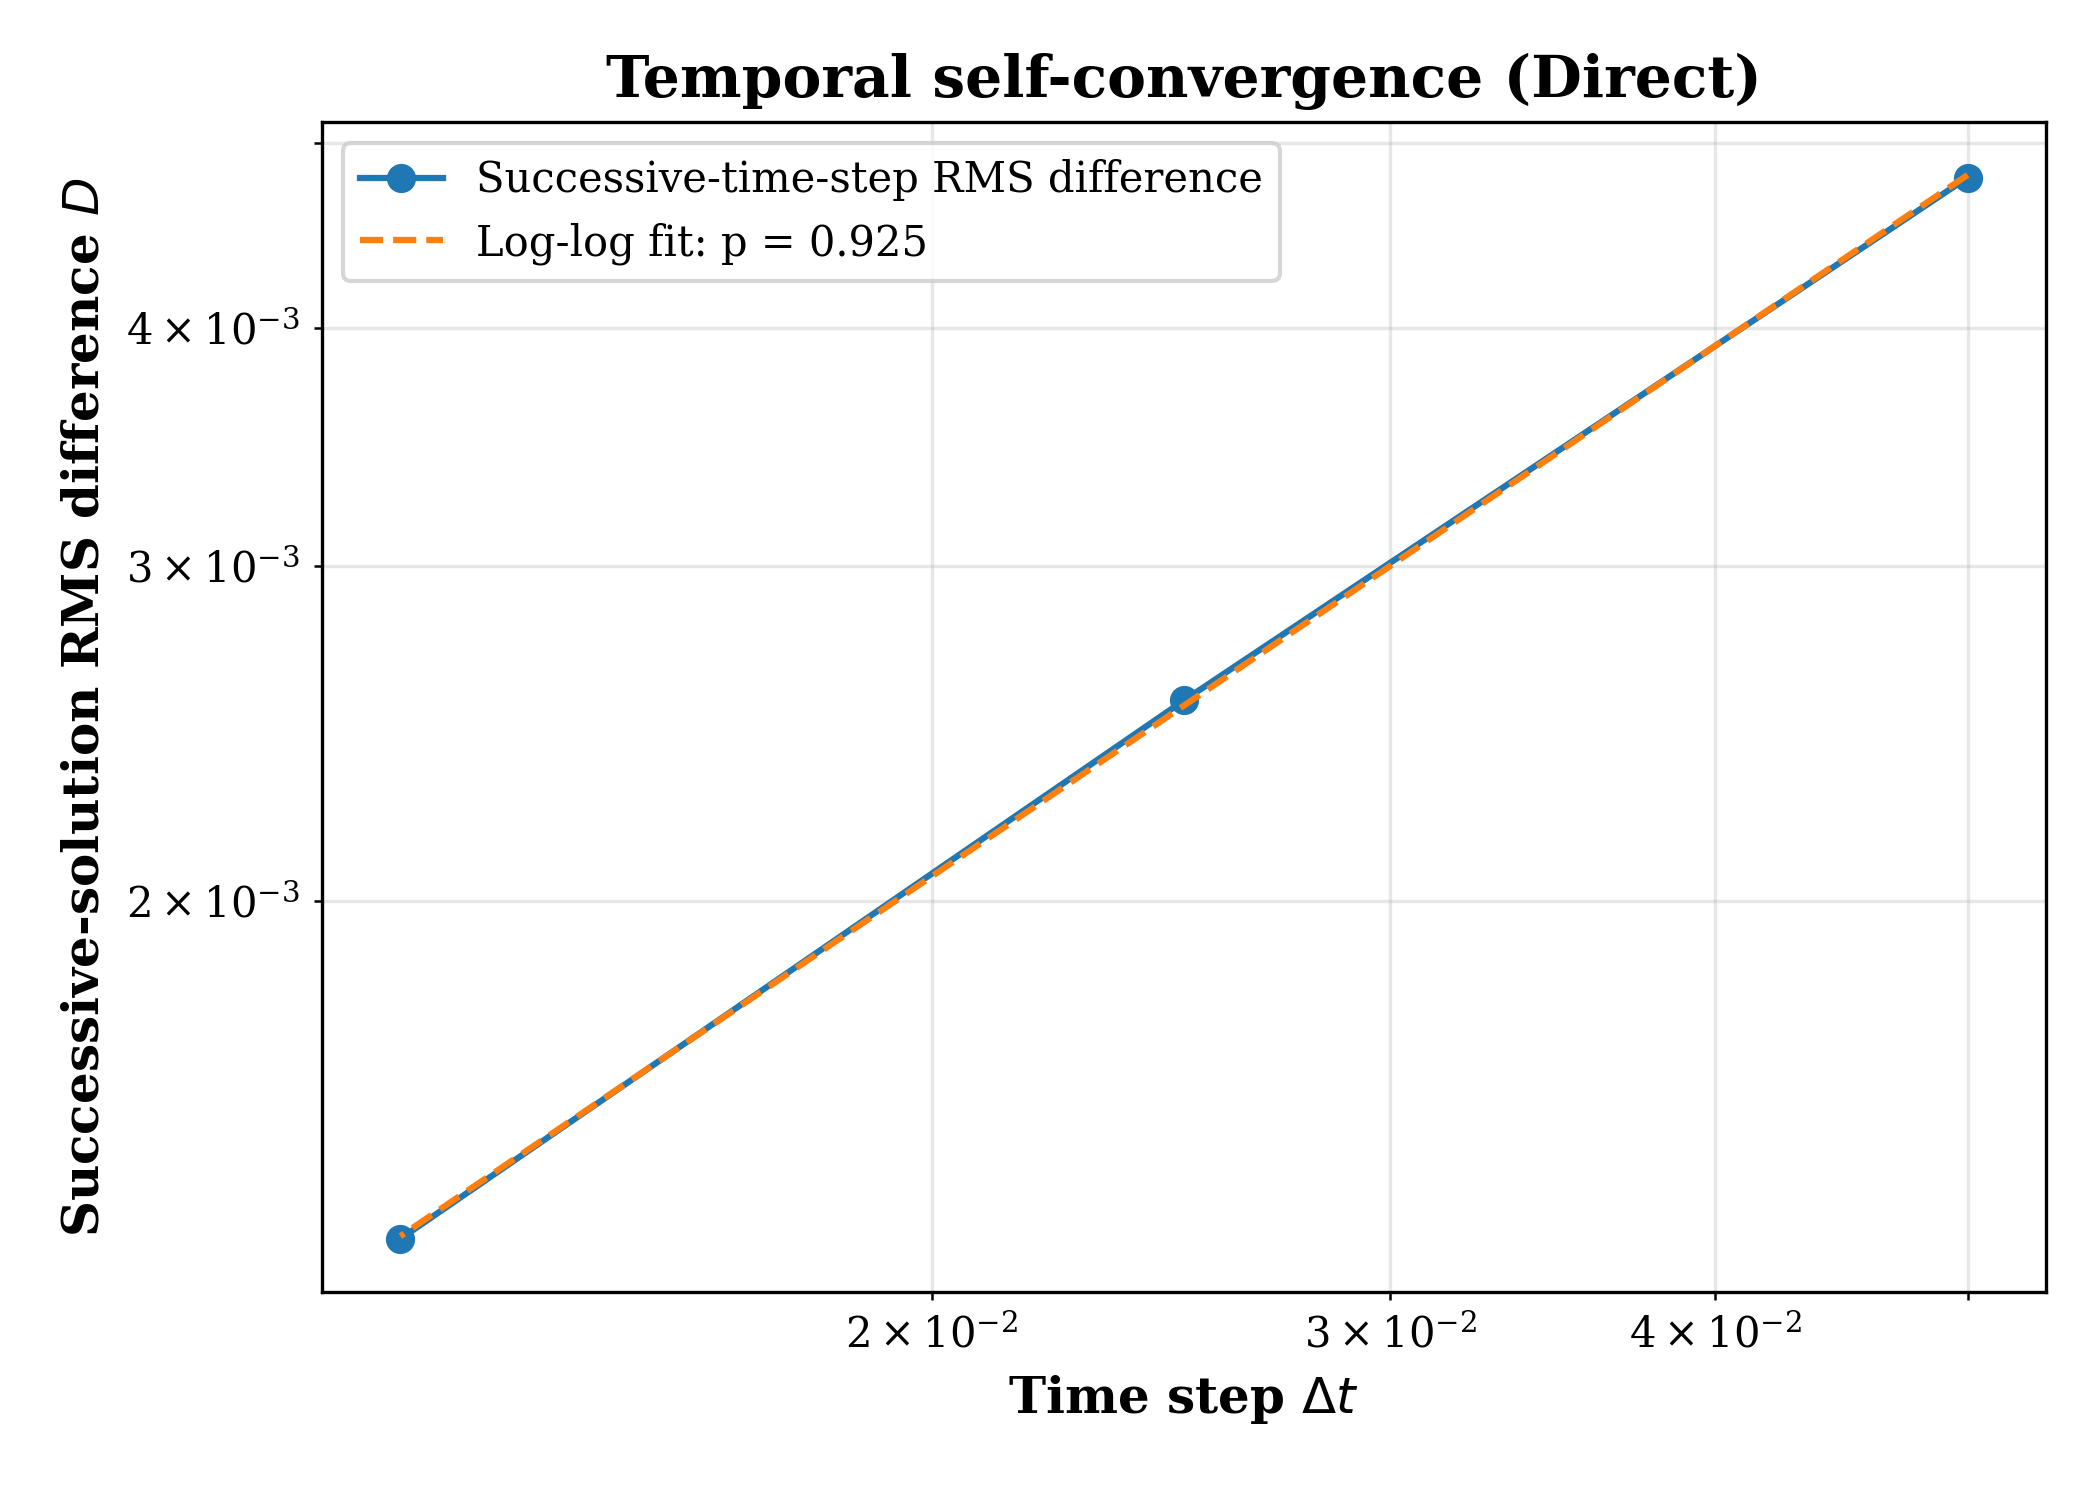
\includegraphics[width=\linewidth]
    {figures/temporal_self_convergence_Direct.png}

    {\small (d) Direct implicit Euler}
\end{minipage}

\caption{Temporal self-convergence of the four numerical
methods on the fixed $25\times10$ grid. Successive-time-step
RMS differences are plotted against the time step on
logarithmic axes.}
\label{fig:temporal_self_convergence}
\end{figure}

The results indicate approximately first-order temporal
convergence for both APF and the direct implicit Euler method,
with fitted orders of $0.93579$ and $0.92488$, respectively.
The explicit midpoint method exhibits approximately
second-order convergence, with a fitted order of $2.07147$.
The classical fourth-order Runge--Kutta method achieves a
fitted order of $4.05646$. These estimates are consistent
with the expected temporal accuracy of the respective
integration schemes.

The successive-difference values also decrease systematically
as the time step is refined. In particular, the RK4 method
exhibits substantially smaller differences than the other
methods for the tested time-step range, consistent with its
higher temporal order. The pairwise estimates for all methods
are reasonably close to their respective theoretical orders,
indicating that the selected time-step range provides a
consistent assessment of temporal convergence.

The final RMS residuals remain approximately between
$0.391$ and $0.393$ for all methods. This is expected because
the calculations are intentionally terminated at the fixed
pseudo-time $\tau_f=0.5$, before reaching steady state.
The residual values therefore characterize the transient
solution at the selected integration horizon and are not
used as a convergence criterion in this study.

Overall, the results confirm the expected temporal orders
of the four numerical methods: first order for APF and
implicit Euler, second order for explicit midpoint RK2,
and fourth order for classical RK4.